\chapter{Results}
\label{chapter:Results}

% low feature graphs
\section{Feature selection versus no feature selection}
\begin{figure}[h]
\begin{center}
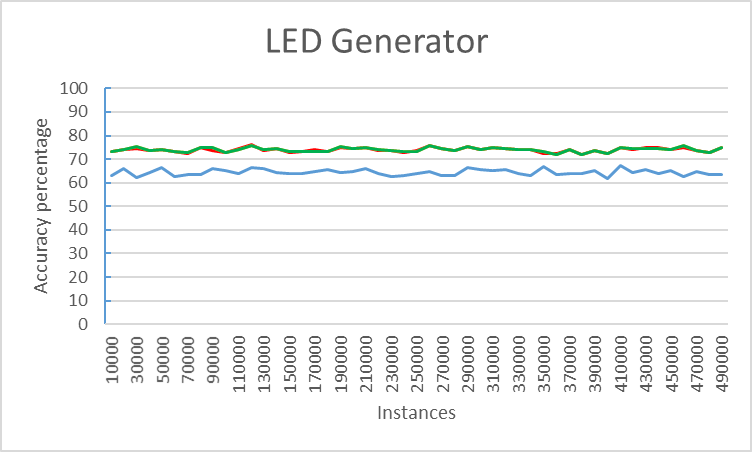
\includegraphics[scale=0.25]{Graphs/LED/10_graph}
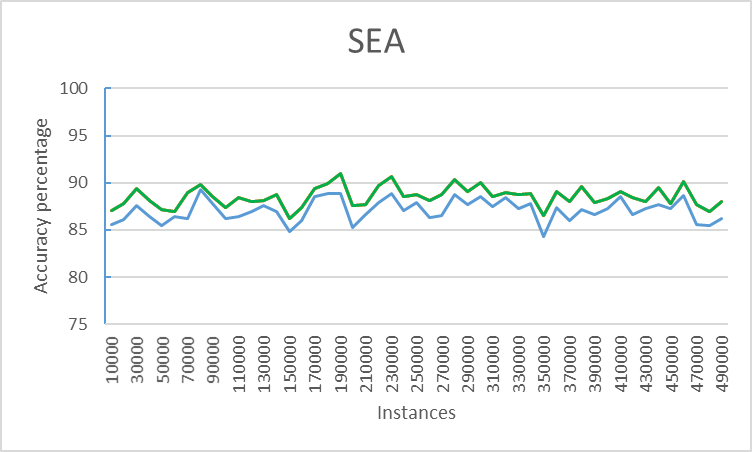
\includegraphics[scale=0.25]{Graphs/SEA/graph}
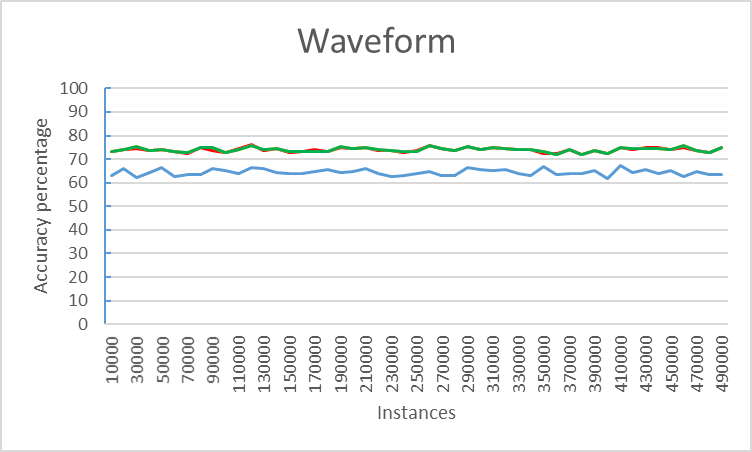
\includegraphics[scale=0.25]{Graphs/Waveform/graph}
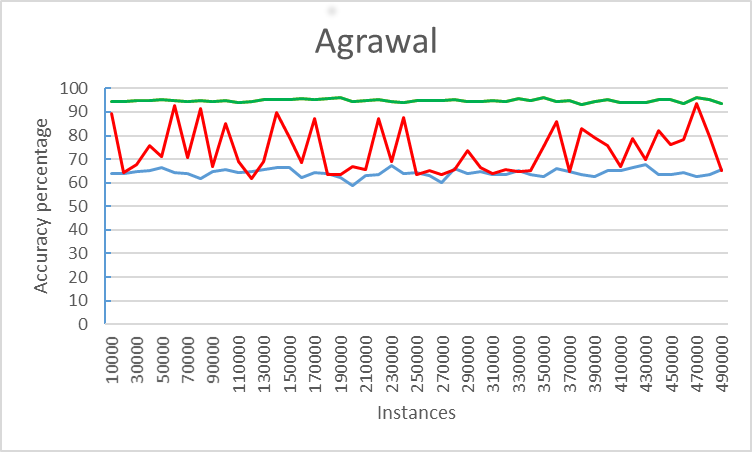
\includegraphics[scale=0.25]{Graphs/Agrawal/graph}
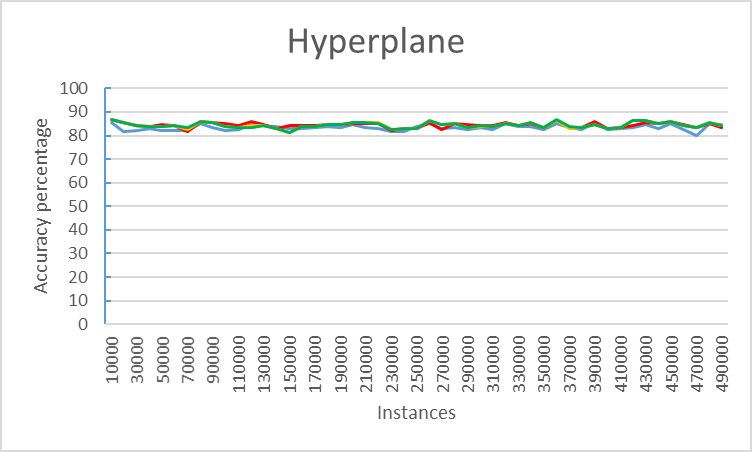
\includegraphics[scale=0.25]{Graphs/Hyperplane/graph}
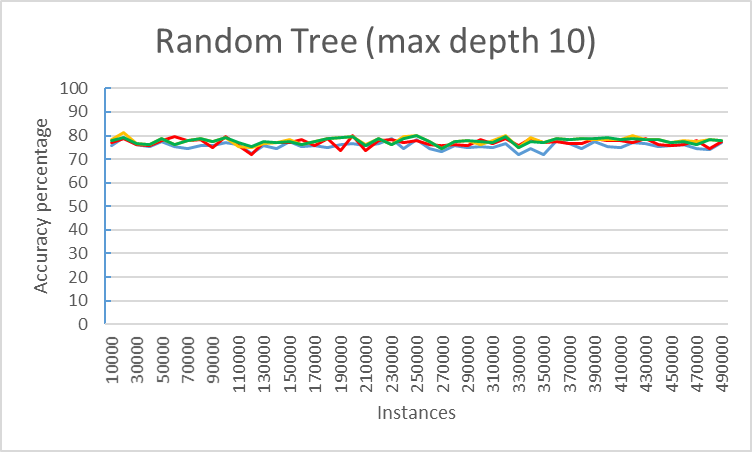
\includegraphics[scale=0.25]{Graphs/TreeD10/graph}
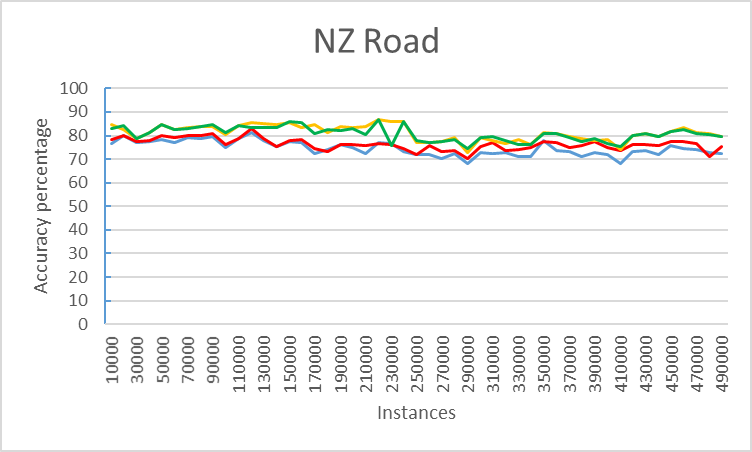
\includegraphics[scale=0.25]{Graphs/NZRoad/graph}

\includegraphics[scale=0.5]{Graphs/legend}
\caption{Prediction Accuracy for static $f$. Lines overlap for some graphs.}
\label{fig:graphs1}
\end{center}
\end{figure}

% fy graphs
\begin{figure}[h]
\begin{center}
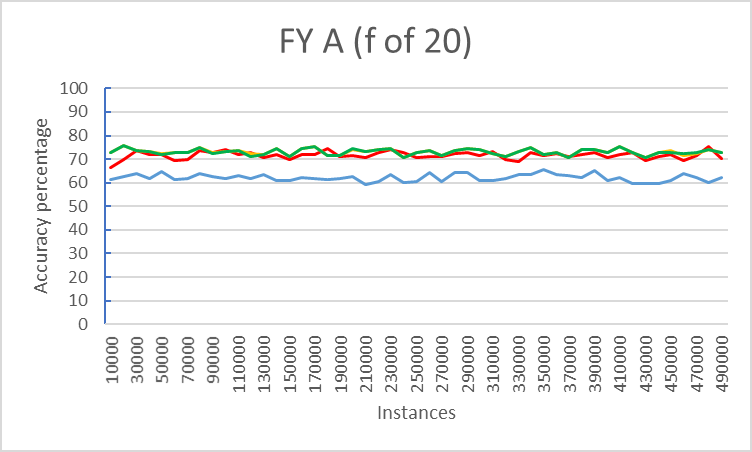
\includegraphics[scale=0.25]{Graphs/FY_A/graph20}
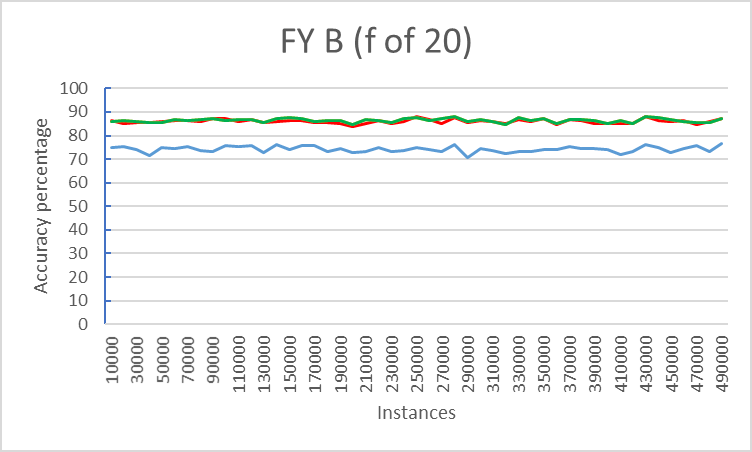
\includegraphics[scale=0.25]{Graphs/FY_B/graph20}
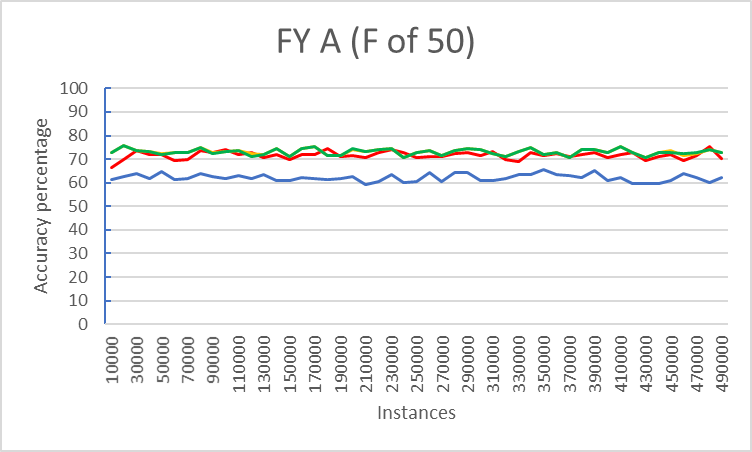
\includegraphics[scale=0.25]{Graphs/FY_A_Drift/graph}
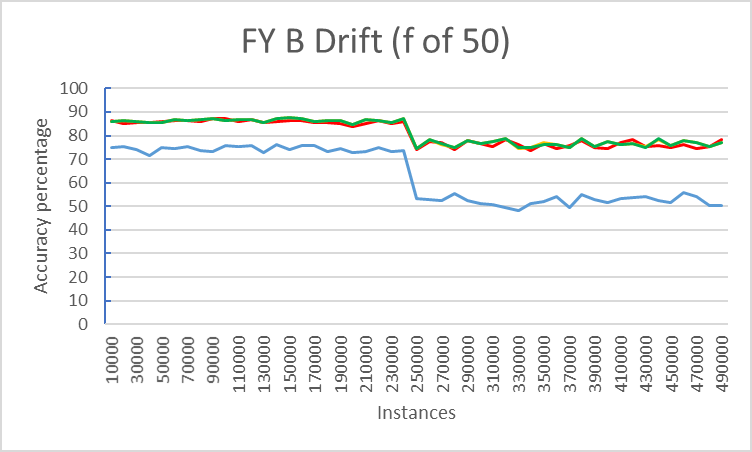
\includegraphics[scale=0.25]{Graphs/FY_B_Drift/graph}
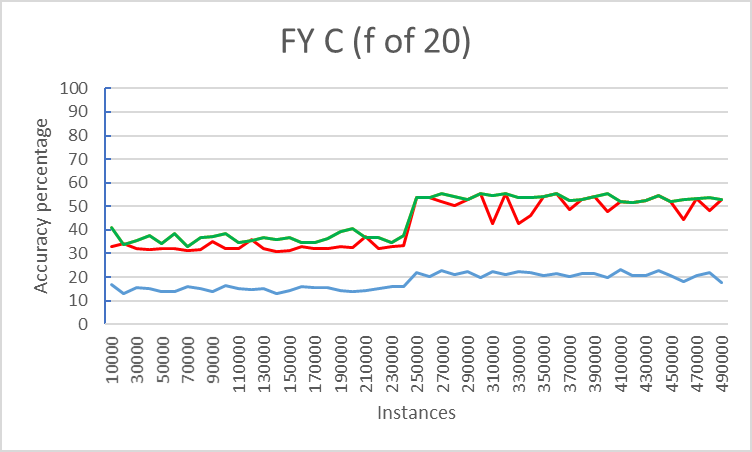
\includegraphics[scale=0.25]{Graphs/FY_C/graph20}
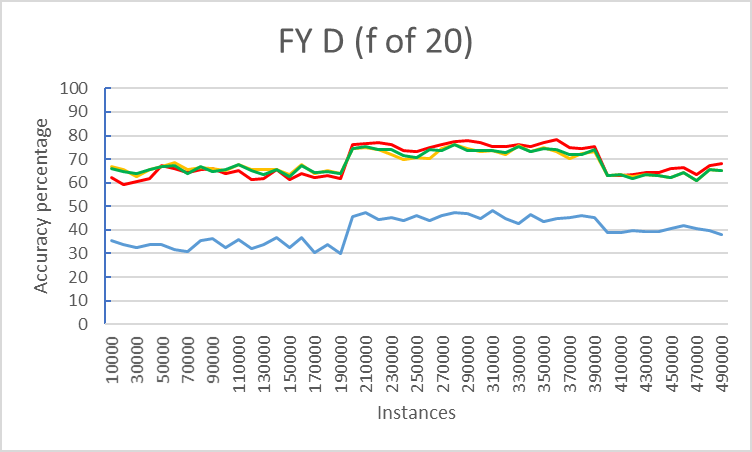
\includegraphics[scale=0.25]{Graphs/FY_D/graph20}

\includegraphics[scale=0.5]{Graphs/legend}
\caption{Prediction accuracy for static $f$.}
\label{fig:graphs2}
\end{center}
\end{figure}

\begin{figure}[h]
\begin{center}
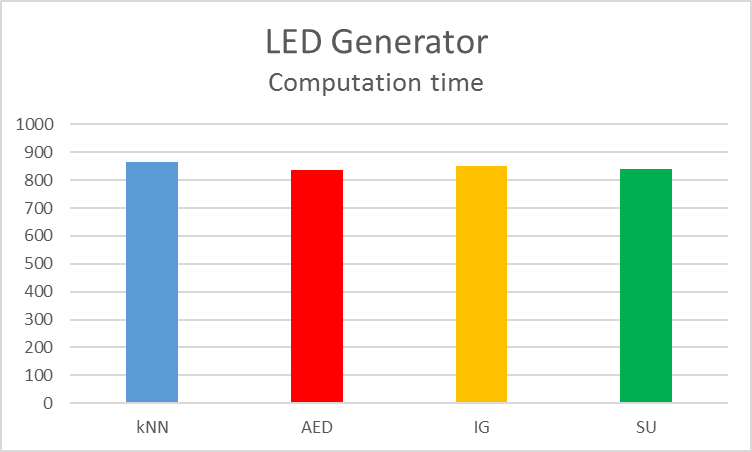
\includegraphics[scale=0.17]{Graphs/LED/10_time}
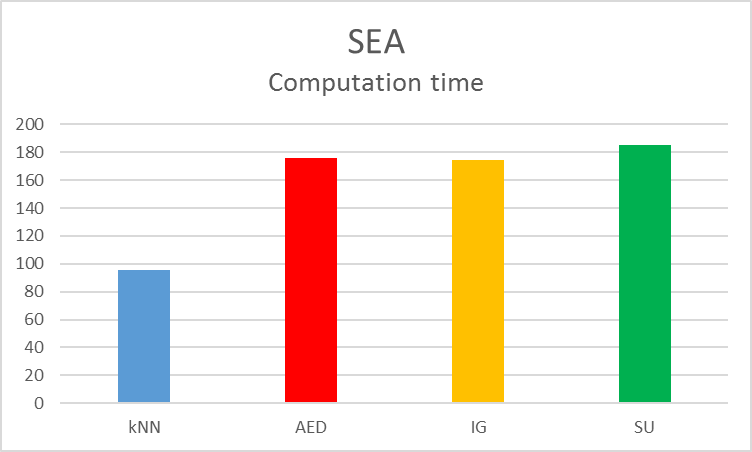
\includegraphics[scale=0.17]{Graphs/SEA/time}
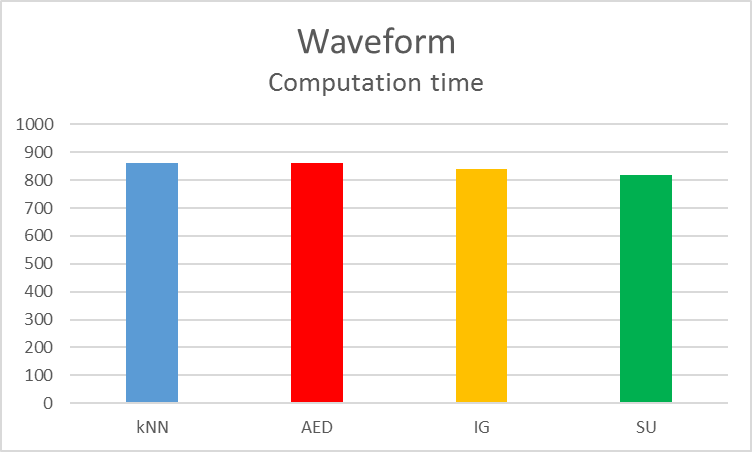
\includegraphics[scale=0.17]{Graphs/Waveform/time}
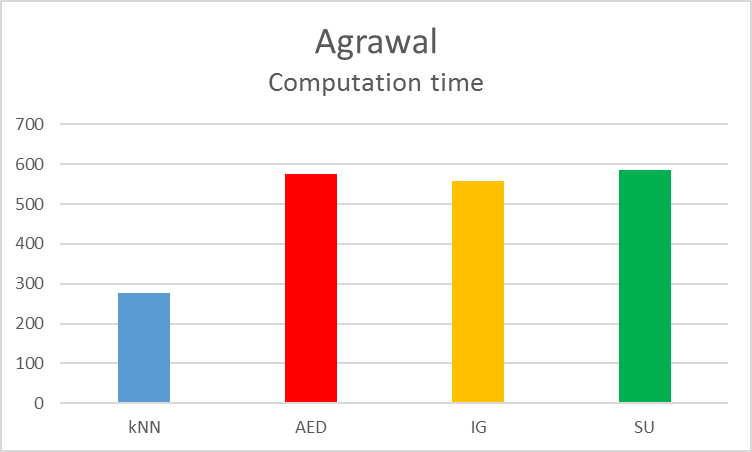
\includegraphics[scale=0.17]{Graphs/Agrawal/time}
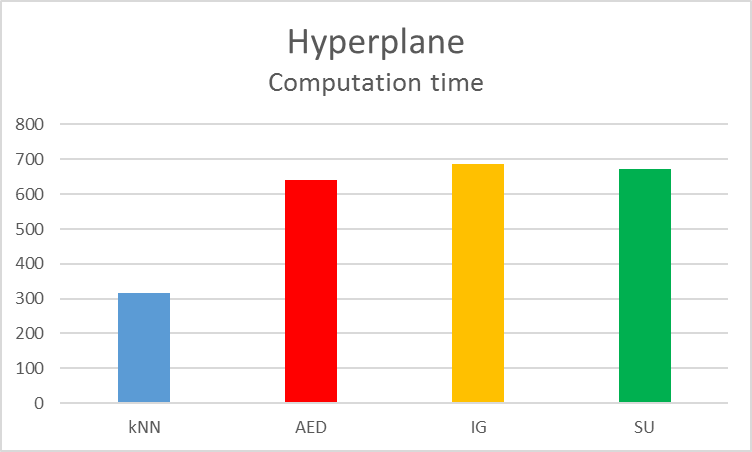
\includegraphics[scale=0.17]{Graphs/Hyperplane/time}
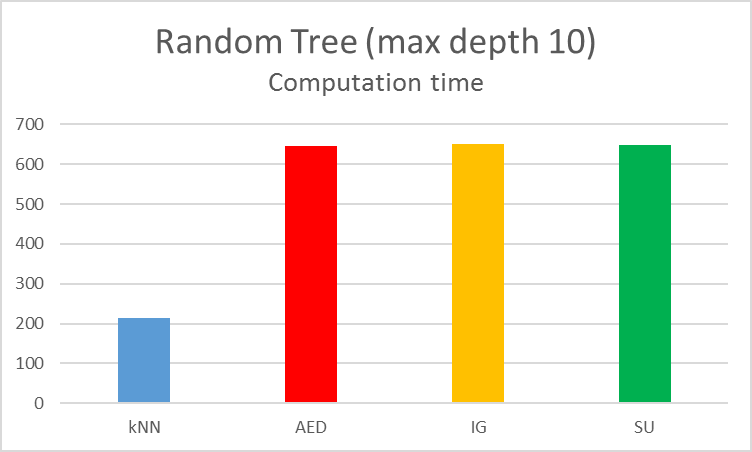
\includegraphics[scale=0.17]{Graphs/TreeD10/time}
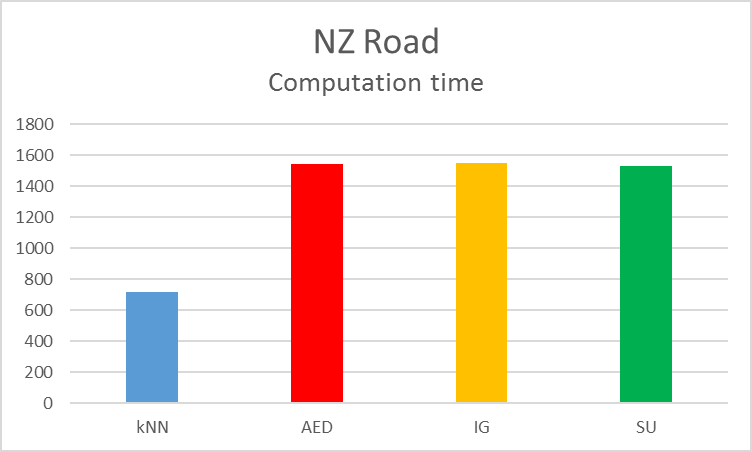
\includegraphics[scale=0.17]{Graphs/NZRoad/time}
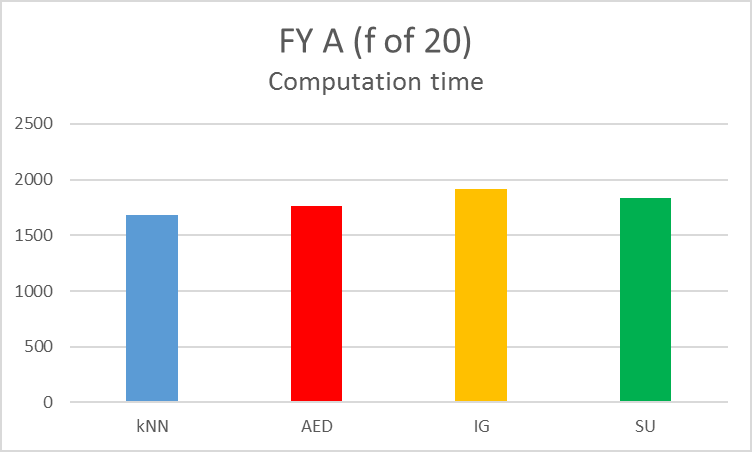
\includegraphics[scale=0.17]{Graphs/FY_A/time20}
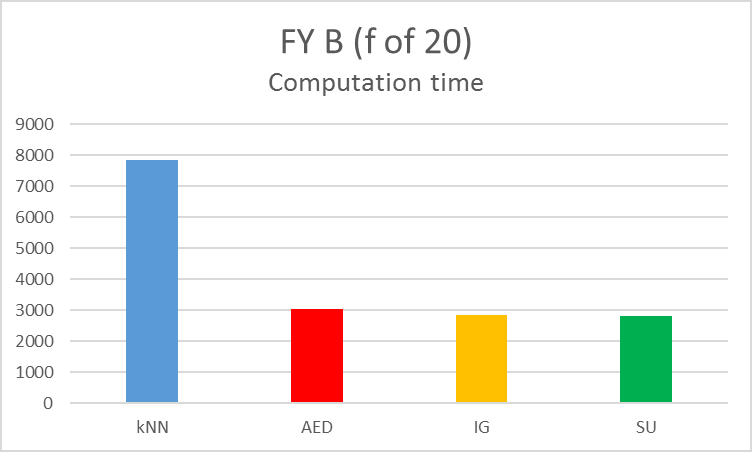
\includegraphics[scale=0.17]{Graphs/FY_B/time20}
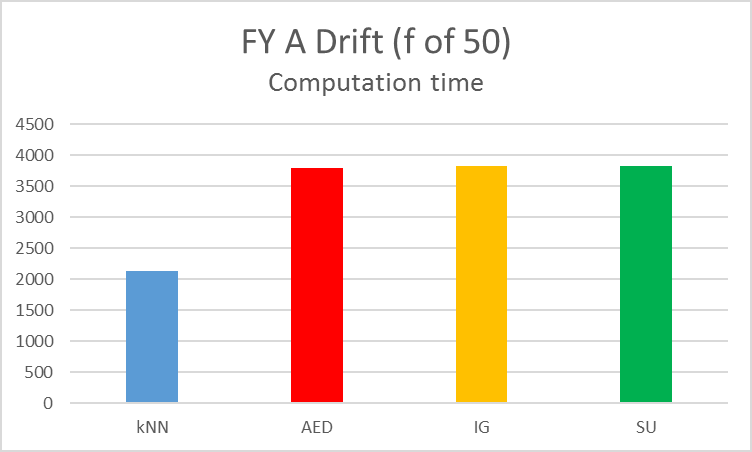
\includegraphics[scale=0.17]{Graphs/FY_A_Drift/time}
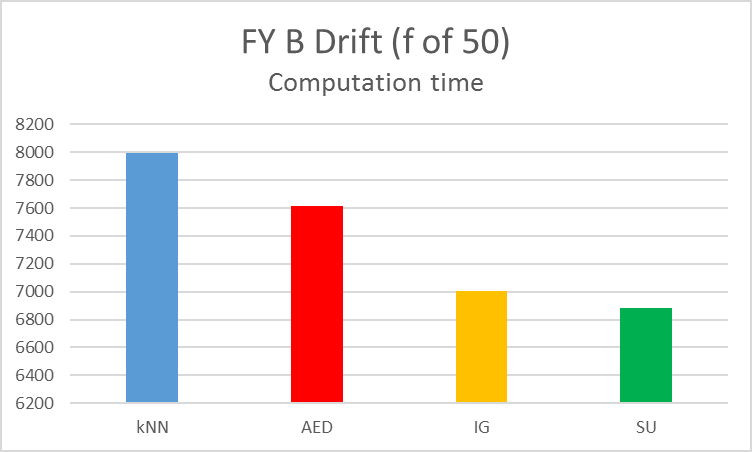
\includegraphics[scale=0.17]{Graphs/FY_B_Drift/time}
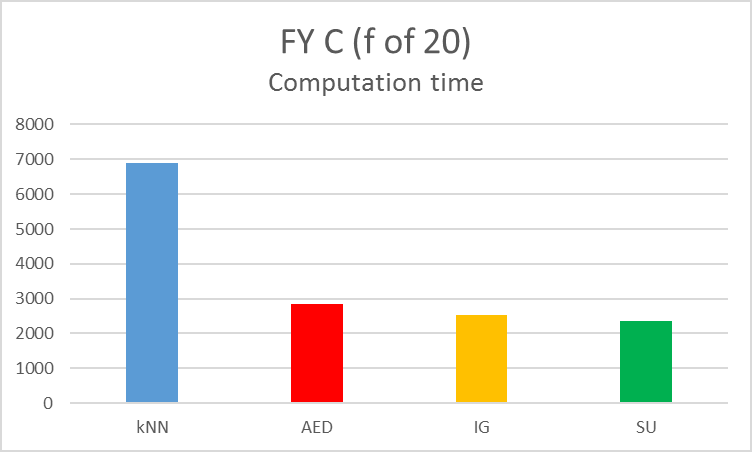
\includegraphics[scale=0.17]{Graphs/FY_C/time20}
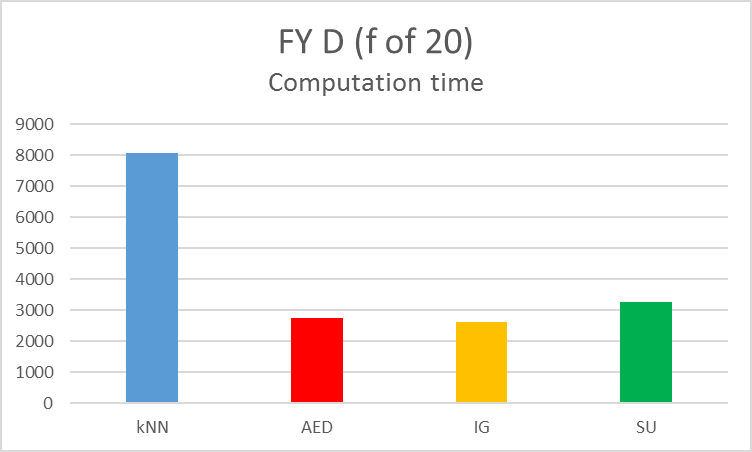
\includegraphics[scale=0.17]{Graphs/FY_D/time20}
\caption{Computation time in seconds of static $f$ experiments.}
\label{fig:time}
\end{center}
\end{figure}

Figure \ref{fig:graphs1} contains prediction accuracy plotted over the stream as new examples come in for static $f$ experiments. Improvements in prediction accuracy can be observed across all experiments when comparing the kNN without feature selection to kNN with feature selection so long as a $f$ of sufficient size was selected. This holds for streams with both a high and low number of features. It was found that selecting a static $f$ too small is detrimental to prediction accuracy as too many features are culled from feature selection, in some cases resulting in worse accuracy than kNN without feature selection. The three ranking functions gave mostly similar results, with SU tending to perform slightly better on average than the other two ranking functions in terms of overall classification accuracy, though not by much. IG and SU ranking functions for the most part performed very similarly to each other due to both being entropy based functions. On experiments such as the Hyperplane and Random tree, the IG and SU lines almost completely overlap each other when plotted on a graph.

In streams without completely irrelevant features such as the Hyperplane and Random tree generators, feature selection was still able to perform with mean accuracies on par with kNN without feature selection so long as $f$ was selected to cover the whole stream. In some cases, very slight improvements (less than 1\%) in mean accuracy were observed for some experiments but were for the most part, marginal and mostly irrelevant. In streams with more irrelevant features, improvement in prediction accuracy over kNN without feature selection is more pronounced. We observed an improvement of roughly 10\% over kNN without feature selection at all times in the LED, Waveform, FY A, and FY B experiments. In the more complex streams (FY C and FY D), very significant improvements were observed with feature selection performing around 30\% better than kNN without feature selection. We also observed that in streams with sudden concept change such as the FY A Drift, FY B Drift, FY C and FY D data sets, the improvement of kNN with feature selection over kNN without feature selection stayed consistent despite drift.

Drifting feature ordering was also tested in the form of the LED Drift and Waveform Drift generators which gave almost identical results to the generators without drift, and hence were not included in graphs. It does however indicate that the feature selection and ranking functions are robust against movements of features' position in the feature space and not biased towards features based on their position in the stream.

Figure \ref{fig:time} shows the time it took for each experiment to complete in seconds. Computation time was found to be highly dependent on the $f$ parameter and how close $f$ is to the actual number of relevant features. How well the ranking function is able to identify the relevant features from the irrelevant features is also important as it impacts on how close $f$ can be set to the actual number of relevant features.

For static $f$ experiments, when $f$ is set close to the actual number of relevant features in a stream with at least some irrelevant features such as in the LED, Waveform, and Conditional generator experiments (FY A, FY B, FY C, and FY D), feature selection outperforms kNN without feature selection in terms of computation time as seen in \ref{fig:time}. This gap widens as the ratio of relevant to irrelevant features increases. In complex streams with more irrelevant features than relevant features as in the FY B, FY C, and FY D, computation time for the best ranking function is around 1/3 that of kNN without feature selection which is a very significant improvement. The three ranking functions had relatively similar computation times, with the AED ranking function seemingly performing faster than the IG and SU ranking functions in streams with more nominal features (such as the SEA and LED experiments) while IG and SU seems to perform faster than AED in streams with more numeric features (such as the Waveform and Hyperplane experiments). Overall, streams with more numeric attributes tended to take longer to compute than those with only nominal attributes due to the added overhead of discretisation for IG and SU, or calculating the mean for AED.

Memory wise, feature selection uses slightly more memory than kNN. The difference is small however with on average 3-6\% increase for the serialised model size. The difference in memory usage is also tied to the types of features in the stream (whether they are nominal or numeric), the features' complexity, and the number of irrelevant features in the stream. The size of $f$ also has an impact on memory usage but the impact is mostly negligible; for example, the experiment on the LED generator used 40 more bytes to construct its model for a $f$ of 20 compared to a $f$ of 10. IG and SU ranking function take the same amount of memory to construct their model in all experiments tested, and tended to in most cases use slightly less memory than the AED ranking function.

\section{Hill climbing $f$ for dynamic subset size selection}

\begin{figure}[h]
\begin{center}
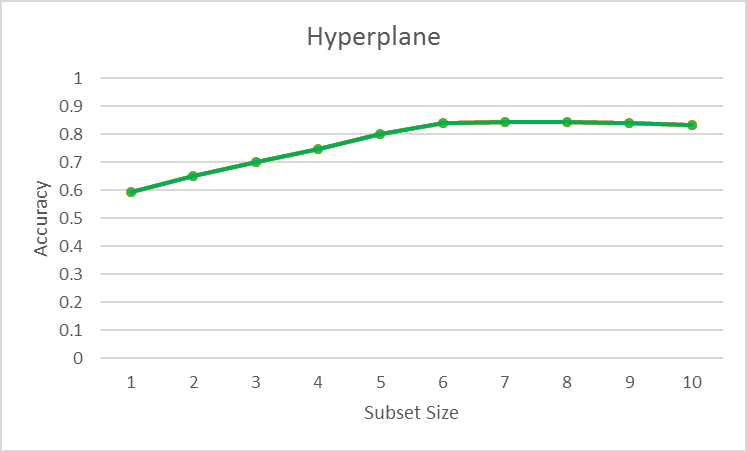
\includegraphics[scale=0.25]{Graphs/AccuracyDifference/Hyperplane}
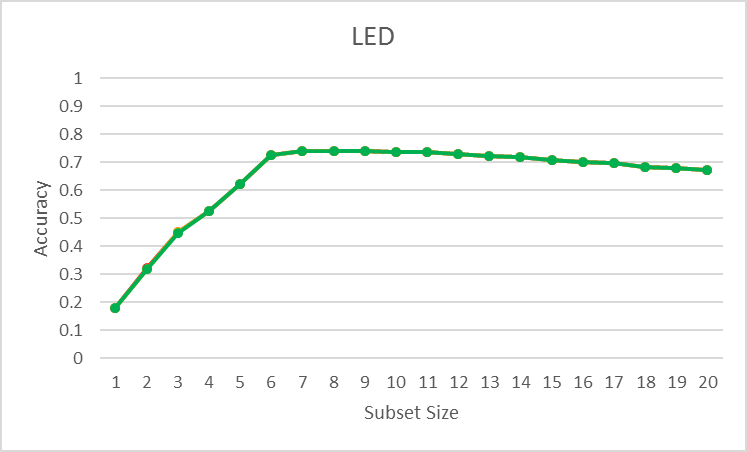
\includegraphics[scale=0.25]{Graphs/AccuracyDifference/LED20}
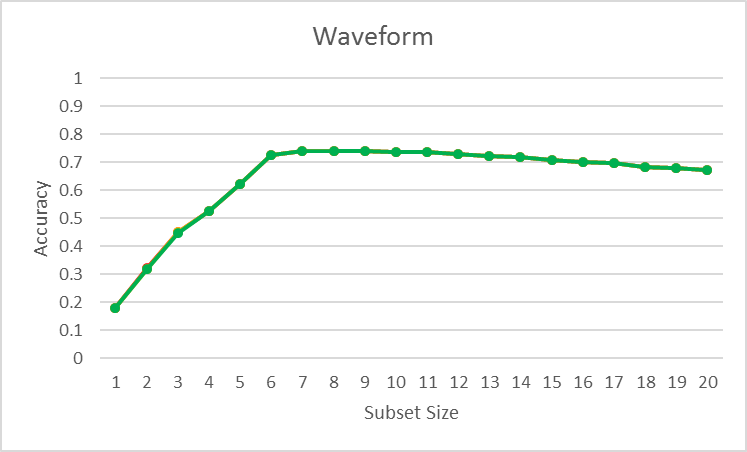
\includegraphics[scale=0.25]{Graphs/AccuracyDifference/Waveform}
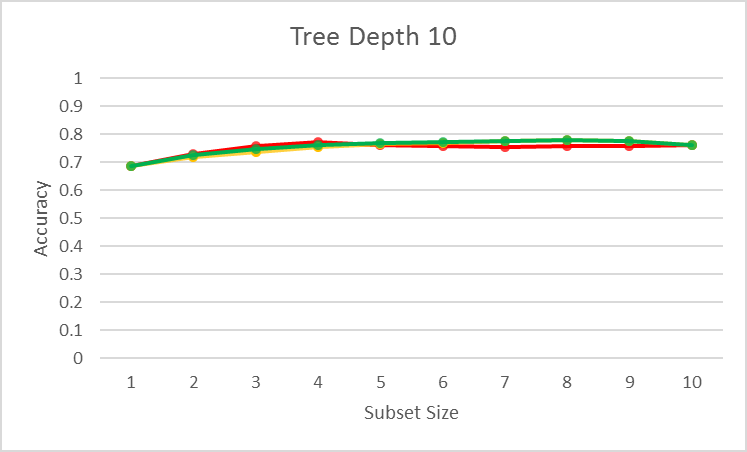
\includegraphics[scale=0.25]{Graphs/AccuracyDifference/TreeD10}
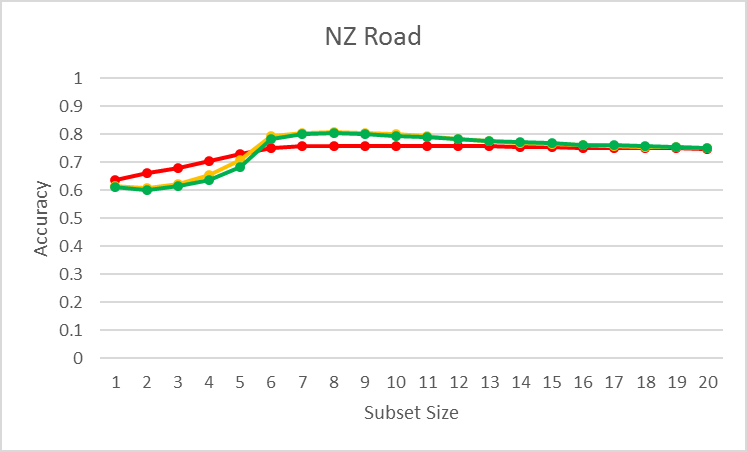
\includegraphics[scale=0.25]{Graphs/AccuracyDifference/NZRoad20}
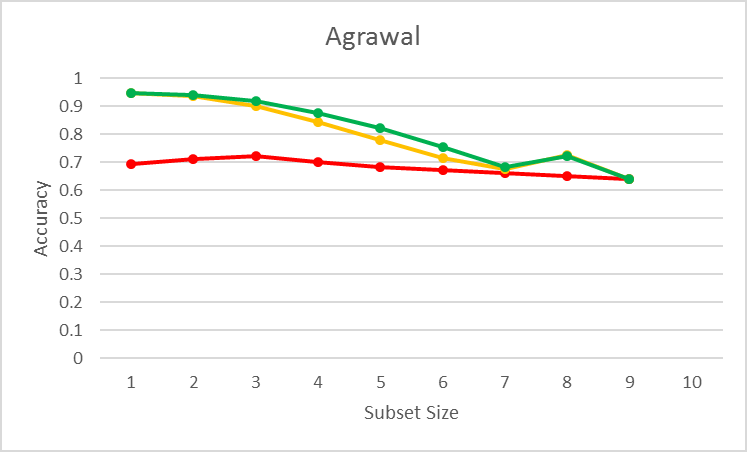
\includegraphics[scale=0.25]{Graphs/AccuracyDifference/Agrawal}
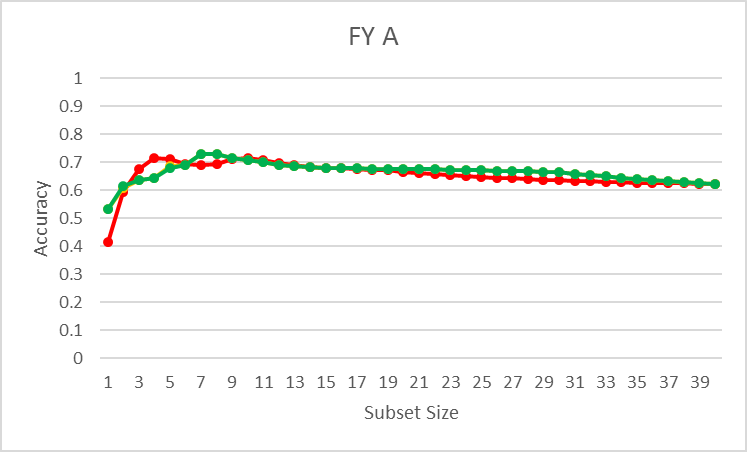
\includegraphics[scale=0.25]{Graphs/AccuracyDifference/FY_A}
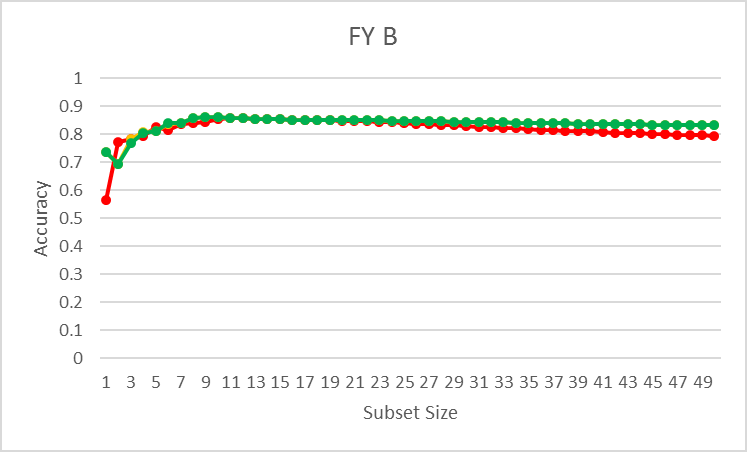
\includegraphics[scale=0.25]{Graphs/AccuracyDifference/FY_B}

\includegraphics[scale=0.5]{Graphs/legendNokNN}
\caption{Average accuracy difference as subset size increases. Lines overlap on some graphs, hence showing only one line.}
\label{fig:accuracyDifference}
\end{center}
\end{figure}

\begin{figure}[h]
\begin{center}
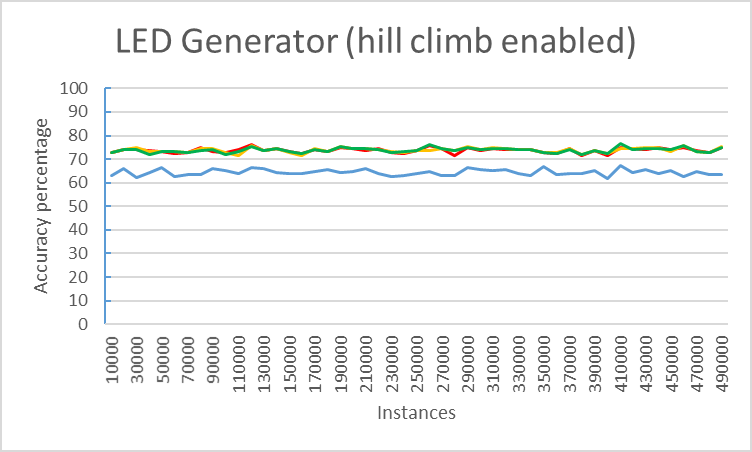
\includegraphics[scale=0.25]{Graphs/LED/H_graph}
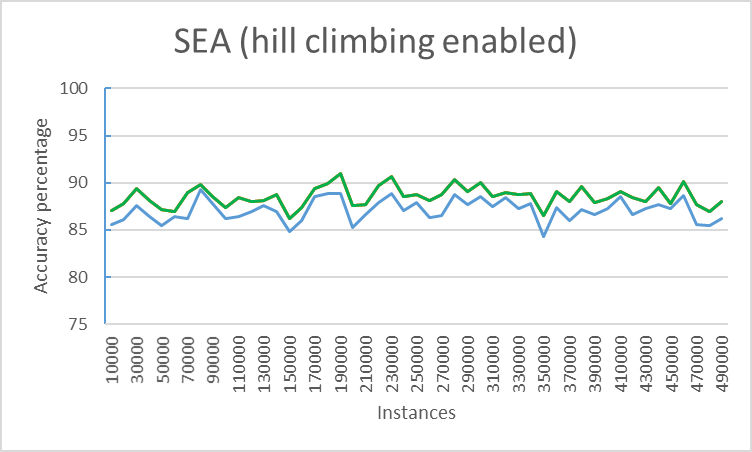
\includegraphics[scale=0.25]{Graphs/SEA/H_graph}
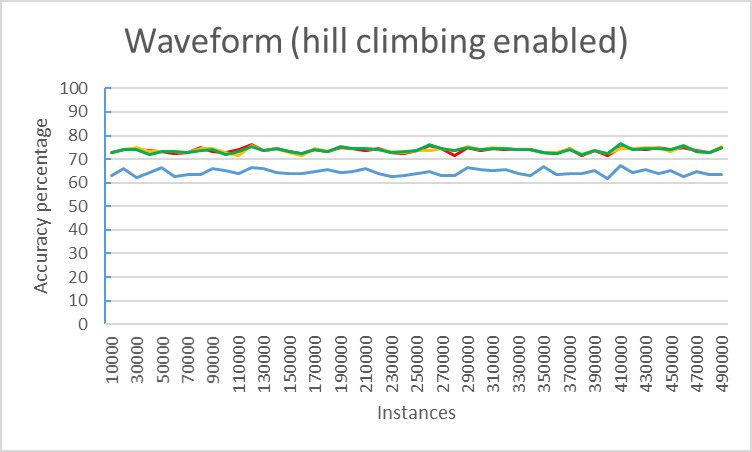
\includegraphics[scale=0.25]{Graphs/Waveform/H_graph}
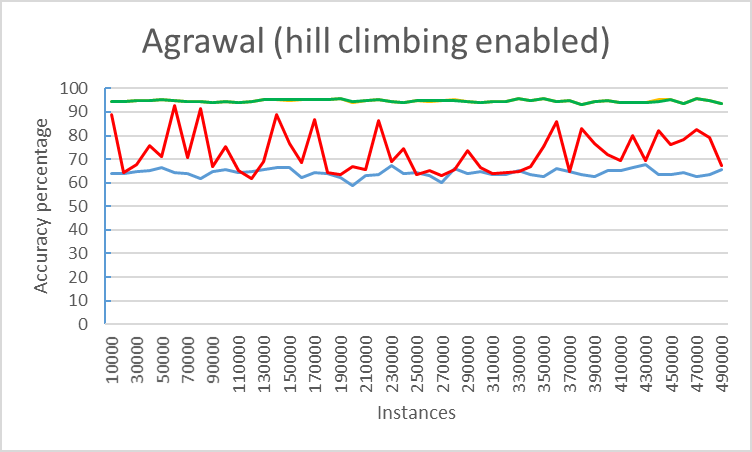
\includegraphics[scale=0.25]{Graphs/Agrawal/H_graph}
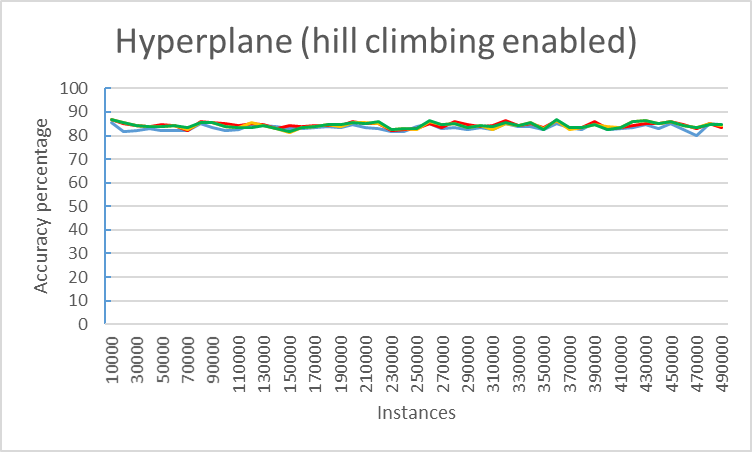
\includegraphics[scale=0.25]{Graphs/Hyperplane/H_graph}
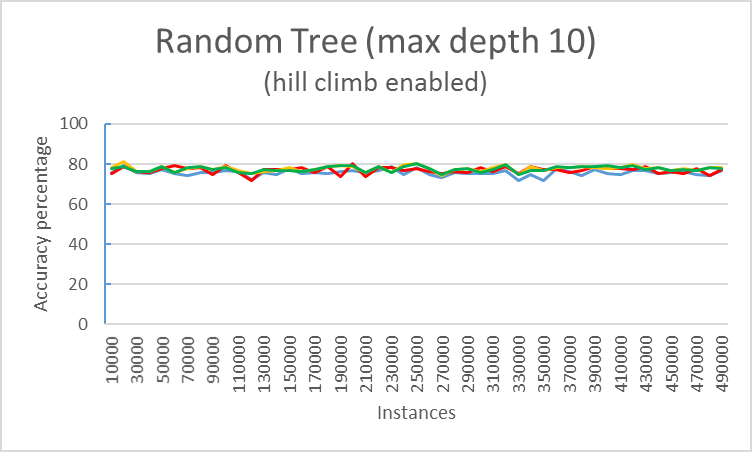
\includegraphics[scale=0.25]{Graphs/TreeD10/H_graph}
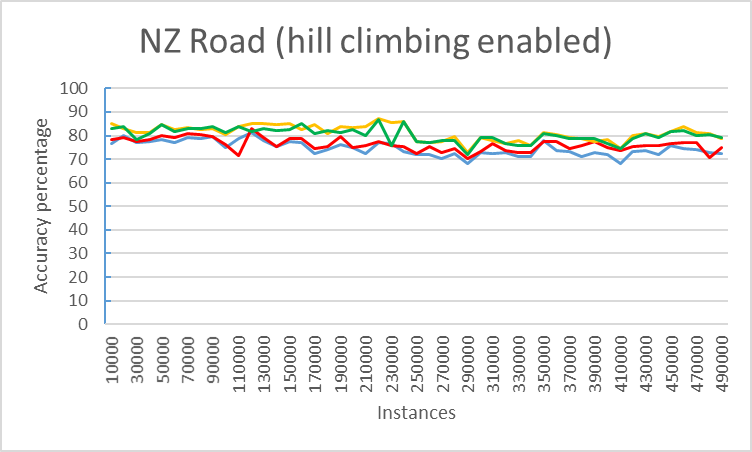
\includegraphics[scale=0.25]{Graphs/NZRoad/H_graph}

\includegraphics[scale=0.5]{Graphs/legend}
\caption{Prediction accuracy for experiments with hill climbing enabled on data streams with a low (less 30) number of features. Lines overlap on some graphs.}
\label{fig:graphs_h}
\end{center}
\end{figure}

\begin{figure}[h]
\begin{center}
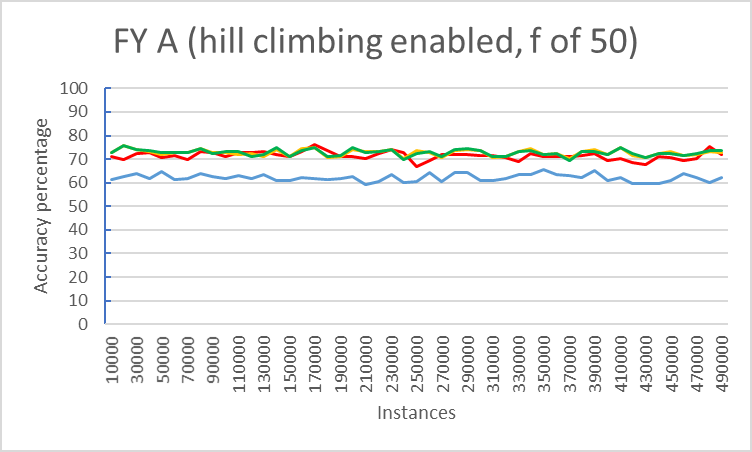
\includegraphics[scale=0.25]{Graphs/FY_A/H_graph}
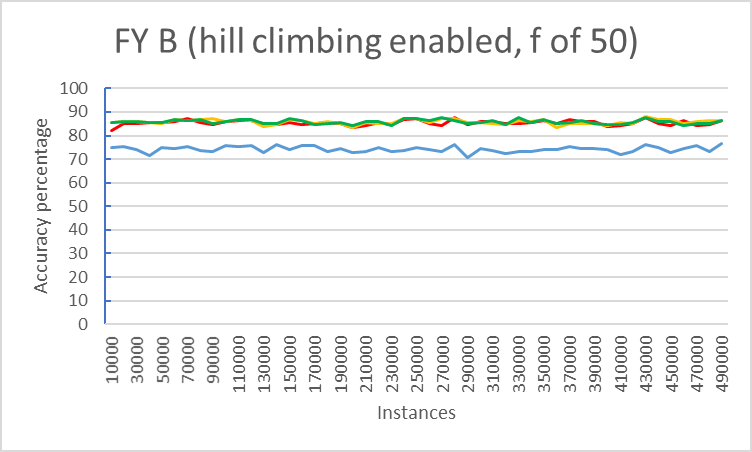
\includegraphics[scale=0.25]{Graphs/FY_B/H_graph}
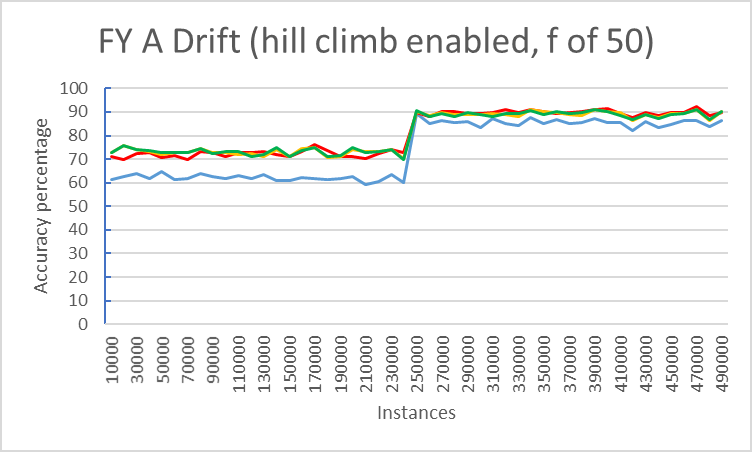
\includegraphics[scale=0.25]{Graphs/FY_A_Drift/H_graph}
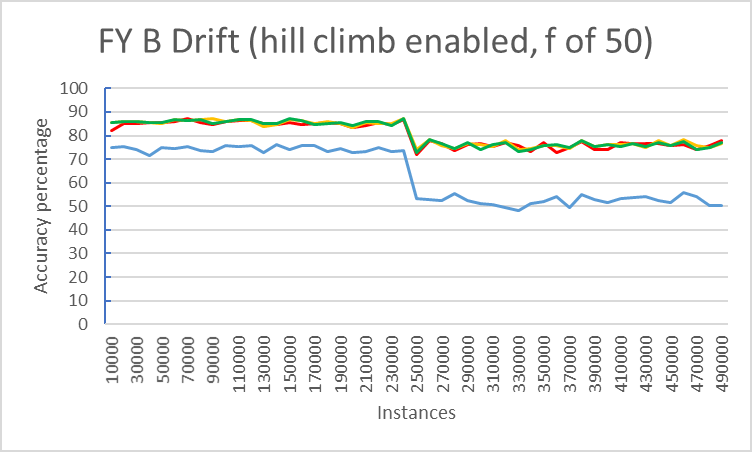
\includegraphics[scale=0.25]{Graphs/FY_B_Drift/H_graph}
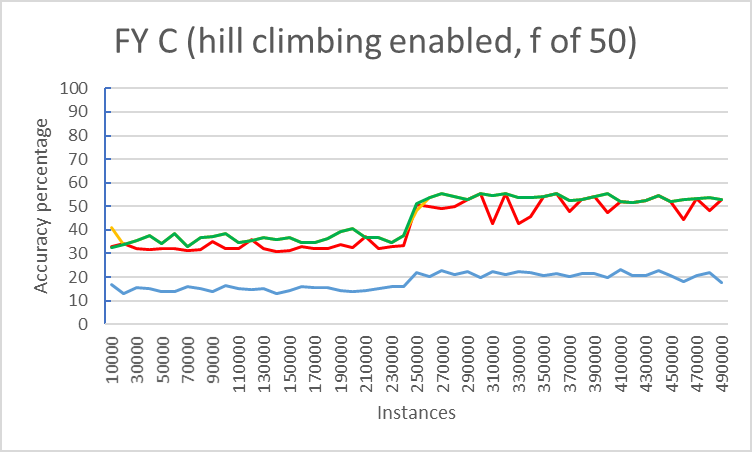
\includegraphics[scale=0.25]{Graphs/FY_C/H_graph}
\includegraphics[scale=0.25]{Graphs/FY_D/H_graph}
\includegraphics[scale=0.5]{Graphs/legend}
\caption{Prediction accuracy for experiments with hill climbing enabled on conditional generator data sets with a high number of features.}
\label{fig:graphs2_h}
\end{center}
\end{figure}



\begin{figure}[h]
\centering 
\includegraphics[scale=0.17]{Graphs/LED/H_time}
\includegraphics[scale=0.17]{Graphs/SEA/H_time}
\includegraphics[scale=0.17]{Graphs/Waveform/H_time}
\includegraphics[scale=0.17]{Graphs/Agrawal/H_time}
\includegraphics[scale=0.17]{Graphs/Hyperplane/H_time}
\includegraphics[scale=0.17]{Graphs/TreeD10/H_time}
\includegraphics[scale=0.17]{Graphs/NZRoad/H_time}
\includegraphics[scale=0.17]{Graphs/FY_A/H_time}
\includegraphics[scale=0.17]{Graphs/FY_B/H_time}
\includegraphics[scale=0.17]{Graphs/FY_A_Drift/H_time}
\includegraphics[scale=0.17]{Graphs/FY_B_Drift/H_time}
\includegraphics[scale=0.17]{Graphs/FY_C/H_time}
\includegraphics[scale=0.17]{Graphs/FY_D/H_time}
\caption{Computation time in seconds of hill climbing $f$ experiments.}
\label{fig:time_h}
\end{figure}

Figure \ref{fig:graphs_h} and \ref{fig:graphs2_h} show the prediction accuracy results for experiments where hill climbing was enabled to dynamically select $f$. In most experiments prediction accuracy suffered a slight decrease when compared to experiments where $f$ is static. The difference however is very small (around 1\% maximum) and generally not impactful. For the same size of $f$, the serialised model size was the same for hill climbing experiments and static $f$ experiments .



\begin{table}[h]
\centering
\begin{tabular}{r|rrr}
						   & No feature selection & Hill climbing $f$ & Static $f$  \\ \hline
LED                        & 863.667   & 616.677    & 840.849   \\
SEA                        & 95.7661   & 183.604    & 185.033   \\
Waveform                   & 862.715   & 613.143    & 818.568   \\
Agrawal                    & 277.674   & 208.513    & 586.588   \\
Hyperplane                 & 314.889   & 539.871    & 673.610   \\
Random Tree                & 214.071   & 488.963    & 649.401   \\
NZ Road                    & 716.659   & 1238.005   & 1533.165  \\
FY A                       & 1681.966  & 780.902    & 1835.689  \\
FY B                       & 7854.827  & 1502.846   & 2811.226  \\
FY A Drift                 & 2134.140  & 958.267    & 1885.345  \\
FY B Drift                 & 7998.333  & 1563.532   & 2743.101  \\
FY C                       & 6890.245  & 806.470    & 2345.209  \\
FY D                       & 8064.495  & 1505.151   & 3275.735 
\end{tabular}
\caption{Comparison of computation time for SU experiments using hill climbing to dynamically select $f$ versus experiments using a static $f$ and experiments with no feature selection.}
\label{Table:H_Time_v_Static}
\end{table}

Figure \ref{fig:time_h} and table \ref{Table:H_Time_v_Static} show the computation time for all experiments conducted. For streams with a highly fluctuating number of relevant features and/or a large number of irrelevant features, as in the FY A, FY B, FY C, and FY D data sets, we observed significant improvements for computation time compared to the static $f$ experiments. The improvement is especially impressive considering the hill climbing experiments had an upper bound of 50 features while the static $f$ experiments considered only the top 20 features, meaning we were able to cover a larger number of features using less time. For streams without many irrelevant features such as the Random tree and Hyperplane generators, hill climbing still performed similarly to static $f$ for computation time and memory usage.

A downside to hill climbing as previously mentioned, is the potential for the algorithm to become stuck in a local optima. If the ranking function was not able to correctly identify and rank the most relevant features above irrelevant features or features detrimental to accuracy, there is a possibility for local optimas to exist. If the hill climbing window is not sufficiently large enough to climb out of the local optimum, the algorithm may get stuck in a suboptimal subset size and prediction accuracy can suffer as a result. One such case can be observed in the FY B data set where the accuracy dips for the IG and SU ranking functions at a subset size of 2, creating a local optima of at subset 1 (This local optimum can be seen on figure \ref{fig:accuracyDifference}). In an extreme case where the hill climbing window is set to 1, the algorithm gets stuck on the local optimum of 1 and considers only one feature for the entire stream; the consequence of which can be seen in figure \ref{fig:stuck_graph}, where both the IG and SU ranking functions' prediction accuracies suffer greatly as a result. However, this is more of an edge case for the entropy based ranking functions and is not replicated in the AED ranking function. A hill climbing window of 2 also alleviates this problem and dislodges the algorithm from the local optima for the entropy based ranking functions. 

The problem still exists however, as simply enlarging the hill climbing window is not an elegant, nor reliable solution. A hill climbing window too large degenerates the algorithm to static $f$ and there is still potential for the algorithm to become stuck even with a very large hill climbing window, though we did not observe any such issue in the experiments we conducted with a hill climbing window of 2.

\begin{figure}[h]
\centering 
\includegraphics[scale=0.25]{Graphs/FY_B/H_graph_stuck}
\includegraphics[scale=0.5]{Graphs/legend}
\caption{FY B with a hill climbing window of 1.}
\label{fig:stuck_graph}
\end{figure}

Despite this potential for getting stuck, we conclude that hill climbing is almost always worth the slight drop in accuracy for the significant improvements in computation time.

\section{Different $k$ sizes}
\begin{table}[h]
\centering
\begin{tabular}{r|rrr}
            & ISS kNN 5 SU & ISS kNN 10 SU & ISS kNN 20 SU \\ \hline
LED         & 73.666   & 73.838    & 73.684    \\
SEA         & 88.012   & 88.514    & 88.554    \\
Waveform    & 73.666   & 73.838    & 73.684    \\
Agrawal     & 94.646   & 94.656    & 94.632    \\
Hyperplane  & 83.122   & 84.396    & 86.106    \\
Random Tree & 77.354   & 77.530    & 77.896    \\
NZ Road     & 80.156   & 80.440    & 80.348    \\
FY A        & 71.344   & 72.768    & 72.788    \\
FY B        & 85.612   & 85.870    & 85.864    \\
FY A Drift  & 80.312   & 81.078    & 80.782    \\
FY B Drift  & 80.442   & 80.804    & 81.522    \\
FY C        & 44.232   & 44.816    & 45.014    \\
FY D        & 66.536   & 67.560    & 68.774
\end{tabular}
\caption{Average prediction accuracy of feature selection using SU ranking with hill climbing enabled for various sizes of $k$.}
\label{Table:K_Table_Accuracy}
\end{table}

We tested our algorithm with different settings for the number of nearest neighbours $k$ to make sure our positive results for a $k$ of 10 was consistent with other sizes of $k$. Due to the constraints of time we only tested the SU ranking function with hill climbing enabled for with different $k$ sizes. $k$ sizes of 5, 10 and 20 were tested. For all sizes of $k$, feature selection continued to show improvements over kNN without feature selection. 

It was observed that overall, the size of $k$ makes a very marginal difference to average prediction accuracy when feature selection was enabled, with a less than 1\% difference in all cases tested. Computation time was somewhat variable in experiments and the results shown in table \ref{Table:K_Table_Time} are the mean computation time of 3 separate experiments for each $k$ size. The general trend observed was that a smaller $k$ tended to compute faster while giving slightly worse accuracy while a larger $k$ gave slightly better accuracy but computed slower. We observed that for some datasets, such as that of the FY B Drift and FY D experiments, the trend is much more pronounced than other experiments. A hypothesis of why this is the case is the different sizes of $k$ cause the hill climbing algorithm to select different sizes of $f$ on those datasets, in which case there would be slightly more or less computation depending on $f$. Memory usage was the same across all $k$ sizes and RAM hours followed the trend shown by computation time.

\begin{table}[h]
\centering
\begin{tabular}{r|rrr}                           
						   & kNN 5 SU & kNN 10 SU & kNN 20 SU \\  \hline
LED                        & 600.023  & 617.875   & 650.041  \\
SEA                        & 183.498  & 185.346   & 186.282  \\
Waveform                   & 600.786  & 620.163   & 649.7603  \\
Agrawal                    & 211.904  & 209.632   & 213.224  \\
Hyperplane                 & 527.956  & 542.545   & 569.375   \\
Random Tree                & 492.952  & 531.496   & 534.947  \\
NZ Road                    & 619.210  & 649.077   & 618.777  \\
FY A                       & 775.961  & 805.683   & 873.682  \\
FY B                       & 1683.483 & 1679.701  & 1849.045  \\
FY A Drift                 & 966.549  & 983.090   & 1055.164  \\
FY B Drift                 & 1487.486 & 1607.153  & 1707.508  \\
FY C                       & 793.588  & 833.257   & 865.196   \\
FY D                       & 1278.419 & 1511.023  & 1811.294
\end{tabular}
\caption{Mean computation time in seconds of feature selection using SU ranking with hill climbing enabled for various sizes of $k$.}
\label{Table:K_Table_Time}
\end{table}


\section{Adaptation to feature drift}
As mentioned in chapter \ref{chapter:RelatedWork}, previous studies have shown feature drift to negatively affect classifier performance in data streams, something feature selection can potentially help address. To test our method's ability to adapt to feature drift, we compared kNN with ISS feature selection to some well know classification algorithms used in stream mining in their ability to adapt to feature drifts. We conducted experiments on 4 data sets created using the Conditional Generator which all contain sudden feature drifts at the halfway point of the stream, except for the FY D dataset, which features two feature drifts at 200,000 and 400,000 instances. The algorithms tested were Naive Bayes (NB), the Hoeffding Tree (VFDT) \citep{Domingos:2000:MHD:347090.347107} and the Hoeffding Adaptive Tree (HAT) \citep{Bifet:2009:ALE:1617420.1617445}.

\begin{figure}[h]
\centering 
\includegraphics[scale=0.25]{Graphs/FeatureDrift/FY_A_Drift}
\includegraphics[scale=0.25]{Graphs/FeatureDrift/FY_B_Drift}
\includegraphics[scale=0.25]{Graphs/FeatureDrift/FY_C}
\includegraphics[scale=0.25]{Graphs/FeatureDrift/FY_D}
\includegraphics[scale=0.5]{Graphs/legendCompareFD}
\caption{Accuracy comparison of various classification algorithms over streams with sudden feature drifts.}
\label{fig:FeatureDrift}
\end{figure}

Figure \ref{fig:FeatureDrift} shows the different algorithms tested on datasets with feature drift. Overall, we observed that kNN based methods appeared to be more resilient to feature drift than the other the algorithms tested with no noticeable dips in accuracy. This is expected behaviour due to kNN's use of the sliding window which allows it to implicitly adapt to change. What is interesting is that ISS appears to amplify simplifications in the stream as seen in the FY C dataset, where after the occurrence of feature drift, the kNN algorithm's accuracy increases by roughly 5\% while the kNN with ISS algorithm's accuracy increases by around 15\%.


\begin{table}[h]
\centering
\begin{tabular}{r|rrr}
          & Mean accuracy & First concept & Second concept \\  \hline
kNN       & 73.876        & 62.132                      & 85.620                       \\
ISS SU HC & 81.078        & 72.988                      & 89.168                       \\
NB        & 79.502        & 87.352                      & 71.652                       \\
VFDT      & 88.110        & 86.740                      & 89.480                       \\
HAT       & 89.142        & 86.288                      & 91.996                      
\end{tabular}
\caption{Mean accuracies for FY A Drift dataset for various classification algorithms.}
\label{Table:Feature_Drift_FY_A_Drift}
\end{table}


\begin{table}[h]
\centering
\begin{tabular}{r|rrr}
          & Mean accuracy & First concept & Second concept \\ \hline
kNN       & 63.324        & 74.316                      & 52.332                       \\
ISS SU HC & 80.804        & 85.852                      & 75.756                       \\
NB        & 69.010        & 92.088                      & 45.932                       \\
VFDT      & 80.048        & 92.164                      & 67.932                       \\
HAT       & 89.184        & 91.988                      & 86.380                       
\end{tabular}
\caption{Mean accuracies for FY B Drift dataset for various classification algorithms.}
\label{Table:Feature_Drift_FY_B_Drift}
\end{table}

\begin{table}[h]
\centering
\begin{tabular}{r|rrr}
          & Mean accuracy & First concept & Second concept \\ \hline
kNN       & 18.020        & 14.928                      & 21.112                       \\
ISS SU HC & 44.816        & 36.012                      & 53.620                        \\
NB        & 40.708        & 47.280                      & 34.136                       \\
VFDT      & 25.486        & 39.356                      & 11.616                       \\
HAT       & 46.012        & 39.244                      & 52.780                       
\end{tabular}
\caption{Mean accuracies for FY C dataset for various classification algorithms.}
\label{Table:Feature_Drift_FY_C}
\end{table}

\begin{table}[h]
\centering
\begin{tabular}{r|rrrr}
          & Mean accuracy & First concept & Second concept & Third concept \\ \hline
kNN       & 39.546        & 33.635                      & 45.410                        & 39.640                       \\
ISS SU HC & 67.560         & 64.085                      & 73.345                       & 62.940                       \\
NB        & 62.036        & 85.580                       & 54.080                        & 30.860                       \\
VFDT      & 42.466        & 76.915                      & 22.390                        & 13.720                       \\
HAT       & 75.822        & 75.730                       & 77.585                       & 72.480                      
\end{tabular}
\caption{Mean accuracies for FY D dataset for various classification algorithms.}
\label{Table:Feature_Drift_FY_D}
\end{table}

Results shown in tables \ref{Table:Feature_Drift_FY_A_Drift}, \ref{Table:Feature_Drift_FY_B_Drift}, \ref{Table:Feature_Drift_FY_C} and \ref{Table:Feature_Drift_FY_D} indicate that in the datasets tested, only the HAT algorithm had similar or better mean prediction accuracies compared to kNN with ISS feature selection; even then the HAT algorithm still exhibits noticeable drops in accuracy for datasets with many irrelevant features such as FY C and FY D. In both cases HAT drops below kNN with ISS after the occurrence of feature drift and takes around 50,000 examples to fully recover to a stable accuracy. 

An interesting observation was that algorithms which outperformed kNN with ISS before the feature drift, such as NB and VFDT, had worse or similar accuracies overall due to the dips in accuracy caused by feature drifts. In the FY D dataset, VFDT's prediction accuracy in fact never manages to stabilise nor recover, and ends with a 13\% prediction accuracy which is very close to the expected value for random guessing (10\%). We also observed that the kNN based algorithms (kNN without feature selection and kNN with ISS) adapted and stabilised much faster than the other algorithms after the occurrence of feature drift, which indicates that the implicit adaptation to feature drift offered by kNN through the use of a sliding window can be advantageous and faster than explicit adaptation in certain data streams.

We can conclude from these results that at least for the data sets tested, ISS  does aid in dealing with feature drifts and is able to make the simple and relatively poor performing kNN algorithm much more competitive with other stream classification algorithms while keeping the advantages of the kNN algorithm in feature drifting streams with many irrelevant features.

\section{Comparison to DFW}
\begin{figure}[h]
\centering 
\includegraphics[scale=0.17]{Graphs/LED/vsDFW}
\includegraphics[scale=0.17]{Graphs/SEA/vsDFW}
\includegraphics[scale=0.17]{Graphs/Waveform/vsDFW}
\includegraphics[scale=0.17]{Graphs/Agrawal/vsDFW}
\includegraphics[scale=0.17]{Graphs/Hyperplane/vsDFW}
\includegraphics[scale=0.17]{Graphs/TreeD10/vsDFW}
\includegraphics[scale=0.17]{Graphs/NZRoad/vsDFW}
\includegraphics[scale=0.17]{Graphs/FY_A/vsDFW}
\includegraphics[scale=0.17]{Graphs/FY_B/vsDFW}
\includegraphics[scale=0.17]{Graphs/FY_A_Drift/vsDFW}
\includegraphics[scale=0.17]{Graphs/FY_B_Drift/vsDFW}
\includegraphics[scale=0.17]{Graphs/FY_C/vsDFW}
\includegraphics[scale=0.17]{Graphs/FY_D/vsDFW}
\includegraphics[scale=0.5]{Graphs/legend2}
\caption{Prediction accuracy of kNN with ISS, kNN with DFW and kNN without feature selection.}
\label{fig:Accuracy_comparason}
\end{figure}

As an aside, we also compared ISS to Dynamic Feature Weighing (DFW). DFW is an algorithm proposed in \citep{Barddal:2016} which uses feature weighing to attempt to address feature drifts in streams. For our experiments, kNN with DFW was configured with a $k$ of 10 and window size of 1000, which is the same for what is used in the experiments for kNN with ISS and kNN without feature selection.

Overall, we observed that ISS performs much better than DFW on the datasets which were tested for this project. We observed better accuracies for ISS over all experiments at almost all points of the streams as shown in figure  \ref{fig:Accuracy_comparason}.

\begin{table}[h]
\centering
\begin{tabular}{r|rrr}
            & ISS SU HC kNN & DFW kNN 10 & kNN    \\ \hline
LED         & 73.838           & 60.630     & 64.404 \\
SEA         & 88.514           & 87.186     & 87.064 \\
Waveform    & 73.838           & 60.630     & 64.404 \\
Agrawal     & 94.656           & 69.442     & 64.194 \\
Hyperplane  & 84.396           & 83.704     & 83.424 \\
Random Tree & 77.530           & 75.690     & 75.690 \\
NZ Road     & 80.440           & 74.774     & 74.656 \\
FY A        & 72.768           & 62.952     & 62.182 \\
FY B        & 85.870           & 75.122     & 74.222 \\
FY A Drift  & 81.078           & 74.864     & 73.876 \\
FY B Drift  & 80.804           & 64.888     & 63.324 \\
FY C        & 44.816           & 18.100     & 18.020 \\
FY D        & 67.560           & 40.270     & 39.546
\end{tabular}
\caption{Average prediction accuracy of kNN with ISS versus kNN with DFW and kNN without feature selection.}
\label{Table:Accuracy_comparason}
\end{table}


\begin{table}[h]
\centering
\begin{tabular}{r|rrr}
            & ISS SU HC kNN & DFW kNN 10 & kNN         \\ \hline
LED         & 616.677          & 1464.050   & 863.667  \\
SEA         & 188.838          & 125.304    & 95.766   \\
Waveform    & 613.143          & 1429.401   & 862.715  \\
Agrawal     & 208.513          & 482.765    & 277.674  \\
Hyperplane  & 539.871          & 482.590    & 314.889  \\
Random Tree & 488.963          & 428.656    & 214.071  \\
NZ Road     & 675.980          & 1238.353   & 716.659  \\
FY A        & 780.902          & 3582.565   & 1681.966 \\
FY B        & 1502.846         & 14999.910  & 7854.827 \\
FY A Drift  & 958.267          & 3647.793   & 2134.140 \\
FY B Drift  & 1563.532         & 14837.190  & 7998.333 \\
FY C        & 806.470          & 13570.790  & 6890.245 \\
FY D        & 1505.151         & 15525.580  & 8064.495

\end{tabular}
\caption{Total computation time of kNN with ISS versus kNN with DFW and kNN without feature selection.}
\label{Table:Time_comparason}
\end{table}

Table \ref{Table:Time_comparason} shows the total computation times for ISS with hill climbing enabled using the SU ranking function versus DFW kNN and kNN without feature selection. It was observed that ISS was faster than DFW kNN in all experiments which contained irrelevant features except the SEA dataset. DFW kNN was also faster for the Hyperplane and Random Tree experiments, which had no irrelevant features. In terms of memory, ISS and DFW kNN had similar usage overall with DFW using around 3.2\% less memory on average based on the results of our experiments which can be seen in table \ref{Table:Mem_comparason}.

\begin{table}[h]
\centering
\begin{tabular}{r|rr}

            & ISS kNN & DFW kNN \\ \hline
LED         & 1481432          & 1450912    \\
SEA         & 441792           & 414096     \\
Waveform    & 1481432          & 1450912    \\
Agrawal     & 686568           & 655416     \\
Hyperplane  & 728096           & 695328     \\
Random Tree & 725696           & 695408     \\
NZ Road     & 1246024          & 1210040    \\
FY A        & 2166616          & 2113976    \\
FY B        & 6245448          & 6139272    \\
FY A Drift  & 2166616          & 2113976    \\
FY B Drift  & 6245448          & 6139272    \\
FY C        & 5839656          & 5648528    \\
FY D        & 6441816          & 6228840 

\end{tabular}
\caption{Serialised model size of kNN with ISS versus kNN with DFW and kNN without feature selection.}
\label{Table:Mem_comparason}
\end{table}


